% SkillLens presentation skeleton (Beamer, 16:9). Compile on Overleaf together with ../report/figures,
% ../report/tables and ../report/architecture.tex (upload them next to this file and fix the paths if needed).
% Every \yaz{...} is a prompt for YOUR words; keep slides short and speak the explanation.
\documentclass[aspectratio=169,11pt]{beamer}
\usetheme{default}
\setbeamertemplate{navigation symbols}{}
\setbeamertemplate{footline}[frame number]
\usepackage[T1]{fontenc}
\usepackage[utf8]{inputenc}
\usepackage{booktabs}
\usepackage{tikz}
\usetikzlibrary{positioning,arrows.meta,fit,backgrounds}
\newcommand{\yaz}[1]{\textcolor{red}{\textbf{[YAZ:} #1\textbf{]}}}
\graphicspath{{../report/}}

\title{SkillLens}
\subtitle{Deep learning-based developer skill assessment and job matching}
\author{\yaz{Adın Soyadın}}
\institute{\yaz{Ders, Bölüm, Üniversite}}
\date{\yaz{Tarih}}
\titlegraphic{
\includegraphics[height=1.3cm]{../../web/img/logo.pdf}}

\begin{document}

\begin{frame}
\titlepage
\end{frame}

% 1. Problem and goal ---------------------------------------------------
\begin{frame}{Problem and goal}
\begin{itemize}
  \item \yaz{İş ilanları uzun ve dağınık: aday hangi becerilerin istendiğini nasıl anlar?}
  \item \yaz{CV'de yazan beceri $\neq$ kanıtlanmış beceri}
  \item \textbf{Research question:} how accurately and how fast do a BiLSTM and a fine-tuned
        DistilBERT extract skill and knowledge spans from the same job ads?
\end{itemize}
\end{frame}

% 2. Data ---------------------------------------------------------------
\begin{frame}{Data: SkillSpan}
\begin{columns}[T]
\column{0.55\textwidth}
\small
\begin{tabular}{lrrr}
\toprule
Split & Sentences & Skill & Knowledge \\
\midrule
Train & 4800 & 2221 & 2969 \\
Val & 3174 & 1070 & 1093 \\
Test & 3569 & 1090 & 1174 \\
\bottomrule
\end{tabular}
\column{0.42\textwidth}
\begin{itemize}
  \item Two BIO layers per sentence
  \item Overlap in 97 train sentences $\rightarrow$ two heads
  \item \yaz{Bir örnek cümle göster}
\end{itemize}
\end{columns}
\end{frame}

% 3. Models -------------------------------------------------------------
\begin{frame}{Two models, one task}
\begin{columns}[T]
\column{0.48\textwidth}
\textbf{BiLSTM}
\begin{itemize}\small
  \item embedding $\rightarrow$ BiLSTM $2\times128$ $\rightarrow$ 2 heads
  \item vocabulary from train only
  \item 1.1M parameters
\end{itemize}
\column{0.48\textwidth}
\textbf{DistilBERT}
\begin{itemize}\small
  \item \texttt{distilbert-base-cased} $\rightarrow$ 2 heads
  \item first-subword labels
  \item 65.2M parameters
\end{itemize}
\end{columns}
\vspace{1em}
\yaz{Neden bu iki model? Aynı değerlendirme: entity-level P/R/F1, aynı test seti}
\end{frame}

% 4. Architecture -------------------------------------------------------
\begin{frame}{Architecture}
\centering
\resizebox{\textwidth}{!}{% System architecture (TikZ). Needs \usepackage{tikz} and \usetikzlibrary{positioning,arrows.meta,fit,backgrounds}.
% Nodes sit on fixed coordinates (cm) so nothing overlaps when the figure is scaled.
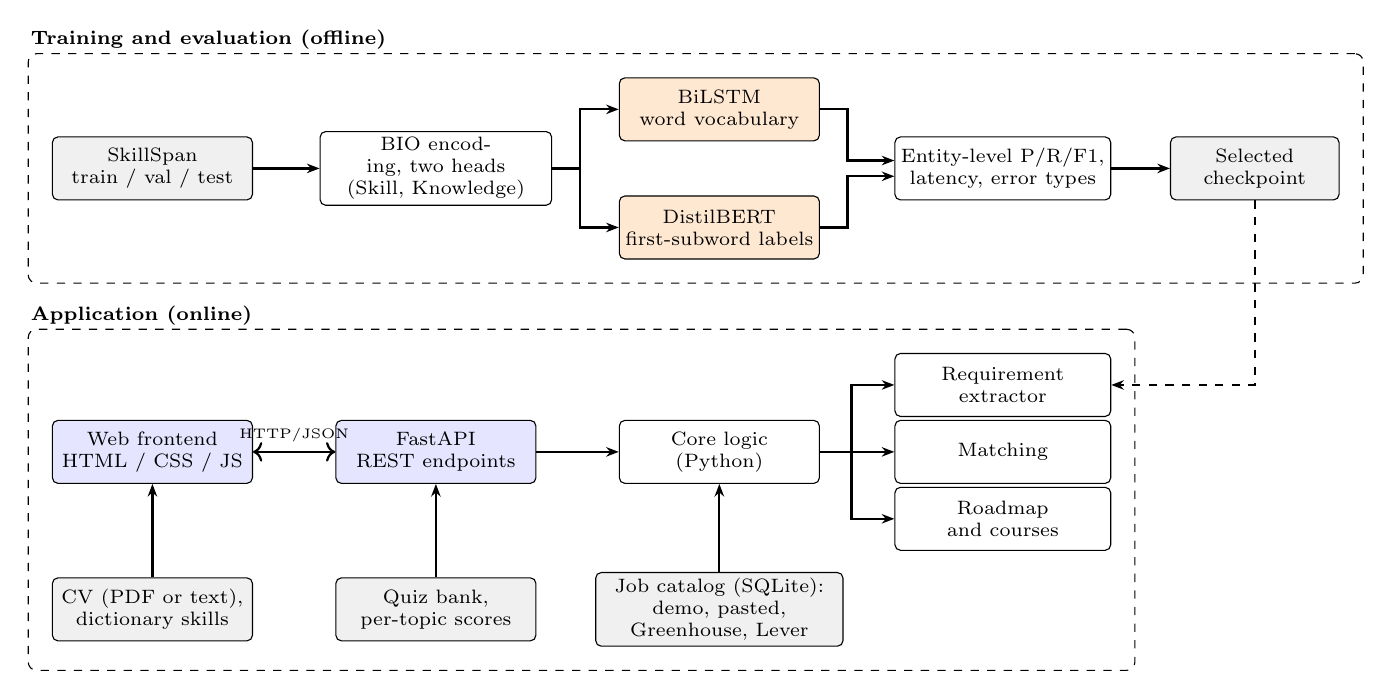
\begin{tikzpicture}[
  font=\scriptsize,
  box/.style={draw, rounded corners=2pt, align=center, minimum height=8mm, text width=#1, inner sep=2pt, fill=white},
  box/.default=24mm,
  data/.style={box=#1, fill=gray!12}, data/.default=24mm,
  model/.style={box=#1, fill=orange!18}, model/.default=24mm,
  app/.style={box=#1, fill=blue!10}, app/.default=24mm,
  arr/.style={-{Stealth[length=1.6mm]}, thick},
  group/.style={draw, dashed, rounded corners=3pt, inner sep=3mm},
  lbl/.style={font=\scriptsize\bfseries, anchor=south west, inner sep=1pt}
]
% ---------------- training and evaluation (offline)
\node[data]          (ss)   at (0, 0)      {SkillSpan\\train / val / test};
\node[box=28mm]      (prep) at (3.6, 0)    {BIO encoding, two heads\\(Skill, Knowledge)};
\node[model]         (lstm) at (7.2, 0.75) {BiLSTM\\word vocabulary};
\node[model]         (bert) at (7.2, -0.75) {DistilBERT\\first-subword labels};
\node[box=26mm]      (eval) at (10.8, 0)   {Entity-level P/R/F1,\\latency, error types};
\node[data=20mm]     (ckpt) at (14.0, 0)   {Selected\\checkpoint};
\draw[arr] (ss) -- (prep);
\draw[arr] (prep.east) -- ++(0.35,0) |- (lstm.west);
\draw[arr] (prep.east) -- ++(0.35,0) |- (bert.west);
\draw[arr] (lstm.east) -- ++(0.35,0) |- ([yshift=1mm]eval.west);
\draw[arr] (bert.east) -- ++(0.35,0) |- ([yshift=-1mm]eval.west);
\draw[arr] (eval) -- (ckpt);
\begin{scope}[on background layer]
  \node[group, fit=(ss)(lstm)(bert)(ckpt)] (train) {};
\end{scope}
\node[lbl] at (train.north west) {Training and evaluation (offline)};

% ---------------- application (online)
\node[app]           (web)   at (0, -3.6)   {Web frontend\\HTML / CSS / JS};
\node[app]           (api)   at (3.6, -3.6) {FastAPI\\REST endpoints};
\node[box]           (core)  at (7.2, -3.6) {Core logic\\(Python)};
\node[box=26mm]      (ext)   at (10.8, -2.75) {Requirement extractor};
\node[box=26mm]      (match) at (10.8, -3.6)  {Matching};
\node[box=26mm]      (road)  at (10.8, -4.45) {Roadmap and courses};
\node[data]          (cv)    at (0, -5.6)   {CV (PDF or text),\\dictionary skills};
\node[data]          (quiz)  at (3.6, -5.6) {Quiz bank,\\per-topic scores};
\node[data=30mm]     (jobs)  at (7.2, -5.6) {Job catalog (SQLite):\\demo, pasted, Greenhouse, Lever};
\draw[arr, <->] (web) -- node[above, font=\tiny] {HTTP/JSON} (api);
\draw[arr] (api) -- (core);
\draw[arr] (core.east) -- ++(0.4,0) |- (ext.west);
\draw[arr] (core) -- (match);
\draw[arr] (core.east) -- ++(0.4,0) |- (road.west);
\draw[arr] (cv) -- (web);
\draw[arr] (quiz) -- (api);
\draw[arr] (jobs) -- (core);
\draw[arr, dashed] (ckpt.south) |- (ext.east);
\begin{scope}[on background layer]
  \node[group, fit=(web)(cv)(jobs)(ext)(road)] (appg) {};
\end{scope}
\node[lbl] at (appg.north west) {Application (online)};
\end{tikzpicture}
}
\end{frame}

% 5. Results ------------------------------------------------------------
\begin{frame}{Results: accuracy}
\begin{columns}[c]
\column{0.55\textwidth}
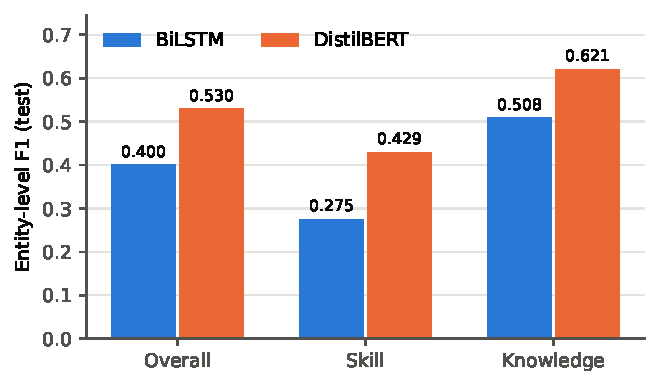
\includegraphics[width=\textwidth]{figures/test_f1.pdf}
\column{0.42\textwidth}
\begin{itemize}\small
  \item DistilBERT F1 0.530 vs BiLSTM 0.400 (seed 42)
  \item 3 seeds: 0.538 $\pm$ 0.008 vs 0.395 $\pm$ 0.006
  \item \yaz{Skill neden daha zor?}
\end{itemize}
\end{columns}
\end{frame}

\begin{frame}{Results: speed and training}
\begin{columns}[c]
\column{0.49\textwidth}
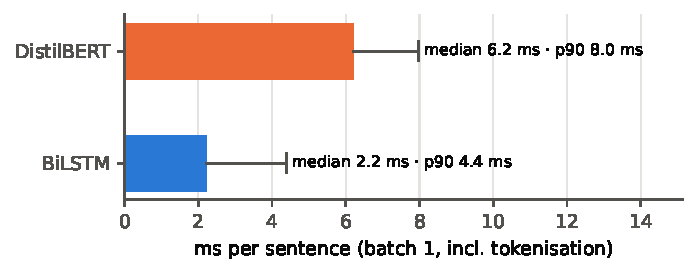
\includegraphics[width=\textwidth]{figures/latency.pdf}
\column{0.49\textwidth}
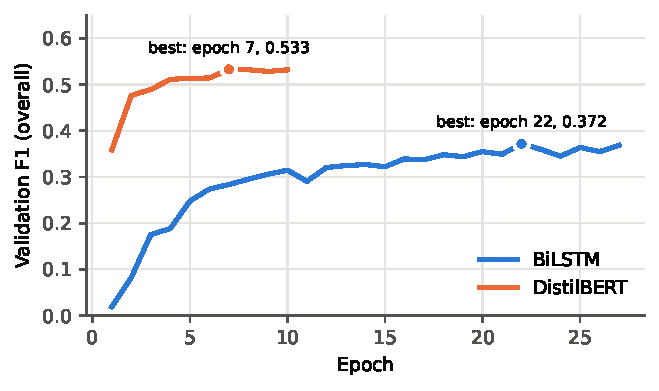
\includegraphics[width=\textwidth]{figures/val_f1_curves.pdf}
\end{columns}
\yaz{Hangi modeli seçtin, neden? (doğruluk vs. hız)}
\end{frame}

\begin{frame}{Error analysis}
\begin{columns}[c]
\column{0.45\textwidth}
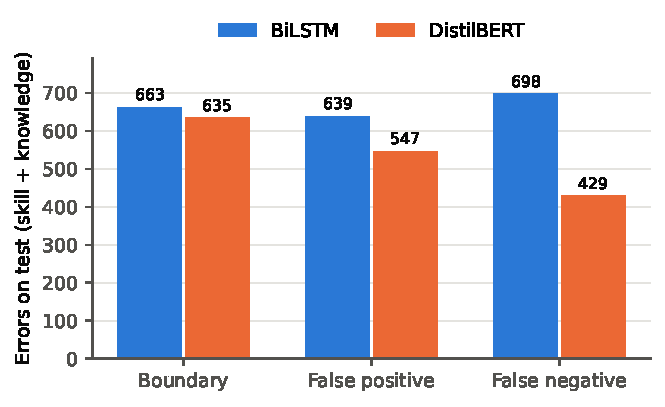
\includegraphics[width=\textwidth]{figures/error_types.pdf}
\column{0.52\textwidth}
\yaz{Tablodan 2 gerçek örnek seç (results/errors\_distilbert.jsonl) ve ne öğrendiğini söyle}
\end{columns}
\end{frame}

% 6. Demo ---------------------------------------------------------------
\begin{frame}{Live demo}
\begin{enumerate}
  \item CV $\rightarrow$ Python, Git
  \item Job: Junior Backend Developer (Python, SQL, Git)
  \item Quiz: Python strong, SQL weak
  \item Match: Git backed by CV, SQL weak
  \item Roadmap: SQL fundamentals + courses
  \item Model lab: paste any job text
\end{enumerate}
\yaz{Demo internet olmadan da çalışıyor; canlı ilan içe aktarma bonus}
\end{frame}

% 7. Conclusion ---------------------------------------------------------
\begin{frame}{Conclusion and limitations}
\begin{itemize}
  \item \yaz{Araştırma sorusunun cevabı, tek cümle, sayılarla}
  \item \yaz{Sınırlamalar: 3 seed, CRF yok, sözlük kapsamı, küçük quiz bankası, sentetik demo ilanlar}
  \item \yaz{Gelecek çalışma}
\end{itemize}
\end{frame}

\begin{frame}
\centering \Large Thank you \\[1em] \normalsize \yaz{Sorular}
\end{frame}

\end{document}
